%% LyX 2.0.3 created this file.  For more info, see http://www.lyx.org/.
%% Do not edit unless you really know what you are doing.
\documentclass[]{CAS}
\usepackage[utf8]{inputenc}
\setcounter{secnumdepth}{3}
\synctex=-1
\usepackage{color}

\usepackage{array}
\usepackage{longtable}
\usepackage{textcomp}
\usepackage{amssymb}
\usepackage{makeidx}
\makeindex
\PassOptionsToPackage{normalem}{ulem}
\usepackage{ulem}
\usepackage{nomencl}
\usepackage[numbers,sort&compress]{natbib} 
\usepackage{hypernat} 
% the following is useful when we have the old nomencl.sty package
\providecommand{\printnomenclature}{\printglossary}
\providecommand{\makenomenclature}{\makeglossary}
\makenomenclature
\usepackage[unicode=true,pdfusetitle,bookmarks=true,bookmarksnumbered=true,bookmarksopen=true,bookmarksopenlevel=2,
 breaklinks=false,pdfborder={0 0 0},backref=false,colorlinks=false] {hyperref}

\makeatletter

%%%%%%%%%%%%%%%%%%%%%%%%%%%%%% LyX specific LaTeX commands.
\providecommand{\LyX}{\texorpdfstring%
  {L\kern-.1667em\lower.25em\hbox{Y}\kern-.125emX\@}
  {LyX}}
%% Because html converters don't know tabularnewline
\providecommand{\tabularnewline}{\\}

%%%%%%%%%%%%%%%%%%%%%%%%%%%%%% User specified LaTeX commands.
\usepackage{tikz}
\usepackage{pgfplots}
\def\oc{\ensuremath{^\circ\hspace{-0.09em}\mathrm{C}}}
%\usepackage{CJKfntef}format=hang 
%\captionsetup[figure]{justification=centering,singlelinecheck=false}
%\captionsetup[figure]{format=hang}
%\usepackage{xstring}
%\raggedbottom

\@ifundefined{showcaptionsetup}{}{%
 \PassOptionsToPackage{caption=false}{subfig}}
\usepackage{subfig}
\makeatother

\begin{document}

\confidential{}


\title{中国科学院博(硕)士学位论文模板}


%\subtitle{——基于Xe\LaTeX{}、\LyX{}与JabRef}


\author{笨笨}


\thesistype{博士学位论文}


\tutor{聪聪\quad{}研究员\quad{}博士}


\tutorinstitute{中国科学院物理研究所}


\institute{中国科学院物理研究所}


\degree{理学博士}


\major{凝聚态物理}


\date{201X年X月}


\institute{中国科学院物理研究所 }


\etitle{\uline{The New UCAS thesis \LaTeX{} template}}


%\esubtitle{\uline{---Case studies of elevated soil warming}}


\eauthor{OMG}


\etutor{GMO}


\emajor{Condensed Matter Physics}


\edegree{Doctor}


\emajortype{Science}


\einstitute{Institute of Physics\\
 Chinese Academy of Sciences }


\edate{June, 201X}

\maketitle

%\Declaration{关于学位论文使用权声明}

%\frontmatter

%这段在正文写作中可以删去或者诊断注释掉,这里只是方便识别版权信息和所有更新说明
\chapter*{致\quad{}谢}

本模板制作过程中参考了清华大学电机工程与应用电子技术系贺凡波制作的清华大学学位论文\LyX{}模板和中国科学院数学与系统科学研究院吴凌云制作的中国科学院学位论文\LaTeX{}模板,在此对作者一并表示感谢。

感谢C\TeX{}论坛LeoLiu的帮助。

感谢中国科学院龙锡恩、leemon albert、陈洪胜和史孝侠帮助测试。

\section*{新的修改}
感谢mgcgogo@gmail.com分享的模板,这个说的真的不错,虽然我不用\LyX{}但是这个模板确实做的非常赞,代码非常简洁、清爽。项目地址\href{http://code.google.com/p/cas-lyx-template/}{http://code.google.com/p/cas-lyx-template/}。

新的中国科学院论文格式要求地址如下:\href{yaoqiu}{http://www.gucas.ac.cn/site/82?u=60473}。这个要求只是限定了封面和封底的格式但是没有要求具体的内容格式,所以我全部保留了mgcgogo的正文及附录部分。如果你的研究所有特别的要求,请参考mgcgogo的介绍自行修改。个人感觉mgcgogo写的介绍真真是极好的。

\today

将整个模板按照中国科学院新的要求进行了更新。有问题请联系shenmingren09@gmail.com。

感谢中国科学院物理研究所何格同学测试Ctex环境。


\begin{abstract}
论文排版对科技工作者来说一直是一个公认的繁琐事情。使用\LaTeX{}排版的突出缺点是控制符和文本符同时显现,容易干扰用户文本内容输入。

鉴于此,,本文提出了一种新颖的\LyX{}+Xe\LaTeX{}+\LaTeX{}组合的论文排版编辑方式。该排版方式取\LyX{}之长弥补\LaTeX{}的不足点,使得同时具有MS
Word和\TeX{}排版两方面优势,同时基于Uincode的Xe\LaTeX{}引擎不仅使得文字兼容性增强,而且使用更方便。本文还以设计一套符合中国科学院博士论文规范的\LaTeX{}/\LyX{}模板为例,验证了该组合方式的可行性。
\end{abstract}

\keywords{中国科学院;\LaTeX{};\LyX{};论文;模板}
\begin{eabstract}
This paper is a thesis template of Chinese Academy of Sciences. A
brief guideline for writing the thesis is also included.
\end{eabstract}

\ekeywords{Chinese Academy of Sciences (CAS); \LaTeX{}; \LyX{}; Thesis; Template }

\tableofcontents{}



\listoffigures


\listoftables


\settowidth{\nomlabelwidth}{排版}
\printnomenclature{}

\mainmatter


\chapter{绪论}

\TeX{}/\LaTeX{}是一种专业的科技文献排版语言,使用它写文档具有如下优势:
\begin{enumerate}
\item 将内容与格式分离,使人专注于内容书写;
\item 编程化控制排版格式,工作灵活性和精确度高;
\item 跨平台,兼容性和稳定性非常好。
\end{enumerate}
但\TeX{}文档没有做到排版控制和内容完全分离。编辑文档时,用户无法避免复杂的\TeX{}/\LaTeX{}命令使用,这会干扰用户输入文章内容,影响思路。

\LyX{}排版软件系统使用户不需直面大量\TeX{}/\LaTeX{}命令,它自动调用\TeX{}/\LaTeX{}引擎最终生成常见的ps、html和pdf等各种常见格式。该系统兼顾\TeX{}与MS
Word排版两者的优势,内容独立于格式的程度非常高。


\section{研究目的}

\begin{figure}[tbph]
\caption{空白图占位用}


\end{figure}


学位论文是典型的科技文献,其具有规范的科技文献排版要求,特别是理工类学位论文需要大量的公式和文档排版。因此研究如何提高学位论文编辑排版工作的效率有非常重要的现实意义。本文结合\LyX{}与\LaTeX{}文档编辑的特点,将\LyX{}与\LaTeX{}用在学位论文编辑排版,研究如何使用这种方法提高论文编辑的效率,最大程度地降低论文排版的繁琐性。


\section{本文的贡献}

本文提出了\LyX{}+Xe\LaTeX{}+JabRef的论文编辑方式。该排版方式取\LyX{}之长弥补\TeX{}/\LaTeX{}的不足,兼具Word和\TeX{}两方面优势,而且基于Uincode的Xe\LaTeX{}引擎不仅使得文字兼容性增强,也令使用复杂度大大降低。

本文以中国科学院博士学位论文为例,设计了一套规范的\LaTeX{}宏和\LyX{}模板,采用Xe\LaTeX{}引擎可一键生成最终PDF文件,用户不必关注底层\LaTeX{}命令。在\LyX{}中\LaTeX{}公式之类的编辑非常方便,所有排版格式化工作由模板完成,用户的集中力在于论文的内容上。

本模板使用起来可以完全的抛开复杂的\LaTeX{}命令%
\footnote{用户实际使用的\LaTeX{}命令只有4个。%
},只需花半个小时的时间学一下\LyX{}的基本操作就可排出规范的学位论文。


\section{用前必读}

本模板使用前一定要搞清楚有没有阻力。论文最后提交到国科图的时候,人家只要PDF文档,这不会有任何问题。但有的导师根本就不知道\TeX{}系统为何物,一看你给他(她)PDF文档,其会抓狂的。一句话:“给我Word版。”……


\chapter{关于本模板}

版本号:1.0%
\footnote{本模板的最新版本可在\href{http://code.google.com/p/cas-lyx-template/}{http://code.google.com/p/cas-lyx-template/}得到。%
}

作者:MGC%
\footnote{作者联系方式:mgcgogo@gmail.com%
}

这是一个用于撰写中国科学院学位论文的\LyX{}模板,名为CAS\LyX{}Thesis。作者将在撰写博士论文的过程中,不断补充和完善本模板。欢迎对本模板或示例文档提出修改意见或指出错误。

\begin{center}
\textbf{声明}
\par\end{center}
\begin{enumerate}
\item 本模板及示例文档不声明任何版权协议,任何个人或团体均可自由使用、修改和发布。由使用本模板而造成的任何损失,模板作者概不负责。
\item 本模板和示例文档为作者根据2012年1月7日中国科学院研究生院颁发的《中国科学院研究生院研究生学位论文撰写规定》和《学位论文编写规则》(GB/T
7713.1-2006)编写而成。“规定”中有明确说明的格式,均按“规定”执行;“规定”中没有明确要求的格式,均按国标执行。 
\end{enumerate}

\section{软件安装与配置}

测试所用软件环境:
\begin{enumerate}
\item Windows 7 + C\TeX{} 2.9.2.159 + \LyX{} 2.0.3 + JabRef 2.7b
\item Debian sid + \TeX{}Live 2011 + \LyX{} 2.0.3 + JabRef 2.7b
\end{enumerate}
模板理论上平台无关,但Mac系统未做测试。\textbf{\textcolor{red}{推荐使用Linux下的\TeX{}Live平台}},个人感觉使用更方便快速。


\subsection{Debian系统的安装}

Debian sid已经包含了\TeX{}Live2011,安装软件只需使用命令:

\texttt{sudo apt-get install texlive lyx jabref}\\
即可。


\subsection{Windows 7系统的安装}

软件下载:
\begin{enumerate}
\item 到 \href{http://www.ctex.org/CTeXDownload/}{http://www.ctex.org/CTeXDownload/}
下载C\TeX{}套装。
\item 到 \href{http://jabref.sourceforge.net/download.php}{http://jabref.sourceforge.net/download.php}
下载JabRef。
\item 到 \href{http://www.lyx.org/Download}{http://www.lyx.org/Download}
下载\LyX{}。
\end{enumerate}
由于安装\LyX{}时,\LyX{}安装程序会检测\cite{PhysRevB.87.184201}系统中的\TeX{}系统,所以安装\cite{RevModPhys.71.1253}顺序应为:C\TeX{}、\LyX{}和JabRef。


\subsection{字体与软件配置}


\subsubsection{字体配置}

本模板的使用中最容易出现问题的地方就是字体了。我们需要用到几种字体:SimSun、SimHei、FangSong、KaiTi、Times
New Roman。Debian下使用命令:

\texttt{fc-list :lang=zh-cn}\\
查看系统中的中文字体。Windows的话,请到系统目录C:\textbackslash{}Windows\textbackslash{}Fonts中查看所需字体。如果没有,从别处复制到Debian系统的\textasciitilde{}/.fonts目录下或Windows的系统字体目录C:\textbackslash{}Windows\textbackslash{}Fonts。不用微软字体的话,则推荐Adobe的那套字体,自己从网上找吧。使用自定义字体,请到模板cls文件的“设置中文字体”处修改对应设置。例如:

\texttt{\textbackslash{}setCJKfamilyfont\{zhhei\}\{SimHei\}}\\
中,后边那个大括号里的“SimHei”指的是你的字体名。你也可以使用字体文件的文件名:

\texttt{\textbackslash{}setCJKfamilyfont\{zhhei\}\{{[}simhei.ttf{]}\}}~\\
注意方括号的使用。

需要注意,XP的仿宋、楷体和WIN 7中的仿宋、楷体不是一码事。XP的仿宋是“仿宋\_GB2312”,WIN 7是“仿宋”,楷体也是如此。


\subsubsection{软件配置}

为了让\LyX{}和JabRef能够交互信息,需设置\LyX{}的\LyX{}Server Pipe路径。菜单Tools-Preferences-Paths-\LyX{}Server
Pipe中设置为:

\texttt{\textbackslash{}\textbackslash{}.\textbackslash{}pipe\textbackslash{}lyxserver}\\
在JabRef菜单选项-首选项-外部程序-插入选中记录引用到\LyX{}/Kile的设置中将路径写为:

\texttt{\textbackslash{}\textbackslash{}.\textbackslash{}pipe\textbackslash{}lyxserver.in}

其实没有这一步\LyX{}也可以正常工作,不过文献多了以后你要从一大堆里边找一个或一组出来,没有JabRef的帮助就不是很方便了。毕竟看着文章题目多选插入才是最直观的。

关于JabRef的更多设置见 \ref{sec:=0053C2=008003=006587=00732E} 节。


\chapter{常用排版示例与模板使用方法}


\section{文档类选项的使用}

本模板的文档类文件CAS.cls中配置了多个文档类选项\index{wdlxx@文档类选项},如a4paper、oneside、twoside之类的无需理会。凡是学位论文中规定死了的,均已在CAS.cls中固定写好。需要使用者调整的有:\index{wdlxx@文档类选项!CJKchapter}CJKchapter、\index{wdlxx@文档类选项!noabcount}noabcount、\index{wdlxx@文档类选项!abGB}abGB和nochaphead\index{wdlxx@文档类选项!nochaphead}。模板默认使用的是中科院规定的格式,也可使用文档类选项对格式进行些许调整。

菜单\texttt{Document -{}-\textgreater{} Settings -{}-\textgreater{}
Document Class -{}-\textgreater{} Class options -{}-\textgreater{}
Custom} 中设置文档类选项,用英文逗号分隔(无顺序要求)。
\begin{description}
\item [{CJKchapter}] 将章标题编号改为中文形式%
\footnote{形如:第一章\quad{}XXXXXX。%
}并居中显示章标题,同时目录和PDF文档的标签也会随之改变。
\item [{noabcount}] 去掉中文摘要后边的图表和参考文献的统计。
\item [{abGB}] 使用国标的摘要格式。
\item [{nochaphead}] 章首页不显示页眉,同时空白页无页眉页脚。
\end{description}
\hspace{2em}当使用选项abGB时,英文摘要的标题为论文的英文标题。论文封面要求英文题目加下划线,模板采用的是在\LyX{}中加入下划线的方式。但这样会造成英文标题变量就是带下划线的,在国标形式的英文摘要中插入英文题目时,该题目也会有下划线,这是不规范的。可做如下调整:
\begin{enumerate}
\item 在CAS.cls文件中搜索“\texttt{\textbackslash{}bf\textbackslash{}san\textbackslash{}@etitle\textbackslash{}\textbackslash{}{[}8pt{]}}”,分别在“\texttt{\textbackslash{}@etitle}”和“\texttt{\textbackslash{}@esubtitle}”前加上命令“\texttt{\textbackslash{}uline}”。
\item 在\LyX{}文件中,将英文标题和英文副标题文本写在Tex命令环境中,并在所有空格前加“\texttt{\textbackslash{}}”。
\end{enumerate}

\section{\index{ct@插图}插图示例}

图形宽度建议为\textbf{7.7cm},图中文字建议使用\textbf{五号字}(\texttt{\textbackslash{}wu})%
\footnote{模板文本宽度为16.4cm,并列图形宽度最好不超过8cm,图中字号应保证全文统一。%
}。


\subsection{单图}

单独的图形示例如图\ref{figg}所示。插入方法为插入浮动图后,在图片位置插入所需图片。一般需要使用段落设置将图形设置为居中,在图形两边插入水平填充也可实现居中。引用图形时,需在图题处插入标签(\texttt{insert
-{}-\textgreater{} label}),在需要引用处插入交叉引用(\texttt{insert -{}-\textgreater{}
cross-reference})。如果图题过长,会自动按悬挂缩进排版。

\begin{figure}[tbph]
\hfill{}\begin{tikzpicture}
\wu
\begin{axis}[width=7.7cm,
ybar,xtick=data,
ylabel=电子数,ymin=0,
symbolic x coords={$<$30keV,30-50keV,50-70keV,70-90keV,$>$90keV},
nodes near coords,
nodes near coords align={vertical},
ymax=9000,
x tick label style={rotate=45,anchor=east},
]
\addplot
coordinates{($<$30keV,7812) (30-50keV,648) (50-70keV,861) (70-90keV,624) ($>$90keV,413)};
legend{ <30keV,30-50keV,50-70keV,70-90keV, >90keV}
\end{axis}
\end{tikzpicture}\hfill{}

\caption[单独图示例]{单独图示例单独图示例单独图示例单独图示例单独图示例单独图示例单独图示例单独图示例单独图示例单独图示例单\cite{1998}独图示例\label{figg}}
\end{figure}


长图题一般没有必要在插图目录中也完整显示,可使用菜单\texttt{Insert -{}-\textgreater{} Short
Title} 插入短标题\index{ct@插图!dbt@短标题}。模板中已将图表编号两边设置了小的间距,不必再手动加入空格。


\subsection{子图}

\index{ct@插图!zt@子图}子图示例如图\ref{fig:=005B50=0056FE=00793A=004F8B}所示。插入方法为,插入浮动图后,在图片位置再次插入浮动图即可。子图亦可单独引用,如图\ref{fig:=005B50=0056FEa}与图\ref{fig:=005B50=0056FEb}所示。

\begin{figure}[tbph]
\hfill{}\subfloat[子图a\label{fig:=005B50=0056FEa}]{\centering{}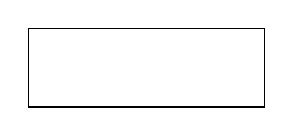
\begin{tikzpicture}
\draw (0,0)rectangle(3,1);
\end{tikzpicture}}\hfill{}\subfloat[子图子图子图子图子图b\label{fig:=005B50=0056FEb}]{\centering{}\begin{tikzpicture}
\draw (0,0)rectangle(3,3);
\end{tikzpicture}}\hfill{}

\caption{子图示例\label{fig:=005B50=0056FE=00793A=004F8B}}
\end{figure}



\subsection{并列图\label{sub:=005E76=005217=0056FE}}

\index{ct@插图!blt@并列图}并列图示例如图\ref{fig:=005E76=005217=0056FE=004E00}与图\ref{fig:=005E76=005217=0056FE=004E8C}所示。插入方法为插入浮动图后,将该浮动图的图题删掉。在浮动图框内插入两个无边框box(\texttt{Insert
-{}-\textgreater{} Box -{}-\textgreater{} Frameless}),右键菜单中设置每个box的宽度为页面宽度的50\%。

\begin{figure}[tbph]
\hfill{}%
\begin{minipage}[t]{0.5\columnwidth}%
\begin{center}
\wu
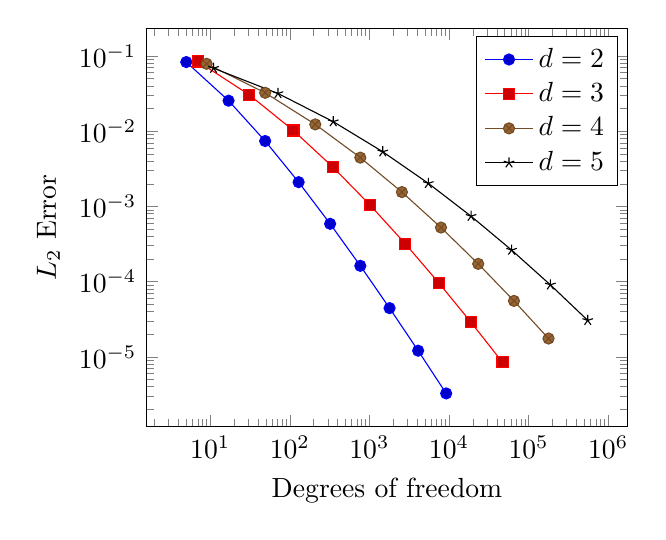
\begin{tikzpicture}
\begin{loglogaxis}[
width=7.7cm,
xlabel={Degrees of freedom},
ylabel={$L_2$ Error}
]
\addplot coordinates{
(5,8.312e-02) (17,2.547e-02) (49,7.407e-03) (129,2.102e-03) (321,5.874e-04) (769,1.623e-04) (1793,4.442e-05) (4097,1.207e-05) (9217,3.261e-06) };
\addplot coordinates{
(7,8.472e-02) (31,3.044e-02) (111,1.022e-02) (351,3.303e-03) (1023,1.039e-03) (2815,3.196e-04) (7423,9.658e-05) (18943,2.873e-05) (47103,8.437e-06) };
\addplot coordinates{
(9,7.881e-02) (49,3.243e-02) (209,1.232e-02) (769,4.454e-03) (2561,1.551e-03) (7937,5.236e-04) (23297,1.723e-04) (65537,5.545e-05) (178177,1.751e-05) };
\addplot coordinates{
(11,6.887e-02) (71,3.177e-02) (351,1.341e-02) (1471,5.334e-03) (5503,2.027e-03) (18943,7.415e-04) (61183,2.628e-04) (187903,9.063e-05) (553983,3.053e-05) };
\legend{$d=2$,$d=3$,$d=4$,$d=5$}
\end{loglogaxis}
\end{tikzpicture} \caption{并列图一\label{fig:=005E76=005217=0056FE=004E00}}

\par\end{center}%
\end{minipage}\hfill{}%
\begin{minipage}[t]{0.5\columnwidth}%
\begin{center}
\wu
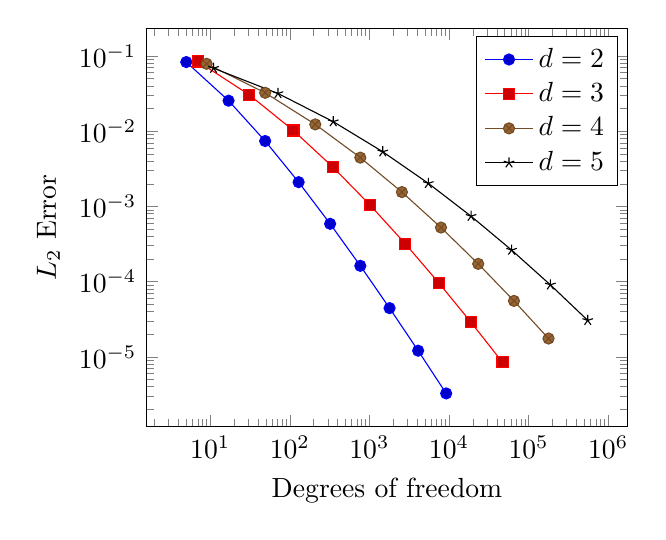
\begin{tikzpicture}
\begin{loglogaxis}[
width=7.7cm,
xlabel={Degrees of freedom},
ylabel={$L_2$ Error}
]
\addplot coordinates{
(5,8.312e-02) (17,2.547e-02) (49,7.407e-03) (129,2.102e-03) (321,5.874e-04) (769,1.623e-04) (1793,4.442e-05) (4097,1.207e-05) (9217,3.261e-06) };
\addplot coordinates{
(7,8.472e-02) (31,3.044e-02) (111,1.022e-02) (351,3.303e-03) (1023,1.039e-03) (2815,3.196e-04) (7423,9.658e-05) (18943,2.873e-05) (47103,8.437e-06) };
\addplot coordinates{
(9,7.881e-02) (49,3.243e-02) (209,1.232e-02) (769,4.454e-03) (2561,1.551e-03) (7937,5.236e-04) (23297,1.723e-04) (65537,5.545e-05) (178177,1.751e-05) };
\addplot coordinates{
(11,6.887e-02) (71,3.177e-02) (351,1.341e-02) (1471,5.334e-03) (5503,2.027e-03) (18943,7.415e-04) (61183,2.628e-04) (187903,9.063e-05) (553983,3.053e-05) };
\legend{$d=2$,$d=3$,$d=4$,$d=5$}
\end{loglogaxis}
\end{tikzpicture} \caption{并列图二\label{fig:=005E76=005217=0056FE=004E8C}}

\par\end{center}%
\end{minipage}\hfill{}
\end{figure}


在box中插入浮动图,此时会显示为子图的样子,现在将浮动图解体(光标定位其中,按del键。),你就会得到并列图形了。可使用水平填充(\texttt{insert
-{}-\textgreater{} formatting -{}-\textgreater{} horizontal space
-{}-\textgreater{} horizoltal fill})在水平方向均匀分布对象,对单一对象直接使用居中即可%
\footnote{模板重新定义了center环境,不会出现间距过大问题。%
}。


\subsection{单页图}

见图\ref{fig:=005355=009875=0056FE=00793A=004F8B}所示。

\begin{figure}[p]
\begin{centering}
\begin{tikzpicture}
\draw (0,0)rectangle(6,19);
\end{tikzpicture}
\par\end{centering}

\caption{单页图示例\label{fig:=005355=009875=0056FE=00793A=004F8B}}


\end{figure}



\section{表格示例}

图题、表题使用的是五号字,对应到\LaTeX{}中的\texttt{\textbackslash{}small},图表中的文字也建议使用五号字。


\subsection{单独表}

\index{bg@表格}表格示例如表\ref{tab:=008868=00683C=00793A=004F8B}所示。在\LyX{}中,选定表格可在右键菜单中对表格进行复杂的设置。

\begin{table}[tbph]
\caption{表格示例\label{tab:=008868=00683C=00793A=004F8B}}


\centering{}%
\begin{tabular}{ccc}
\hline 
\texttt{\small 是} & \texttt{\small 的} & \texttt{\small 是}\tabularnewline
\hline 
\texttt{\small 1} & \texttt{\small abc} & \texttt{\small DEF}\tabularnewline
\texttt{\small 2} & \texttt{\small 234} & \texttt{\small 13.2}\tabularnewline
\hline 
\end{tabular}
\end{table}



\subsection{子表}

表\ref{tab:=005B50=008868=00793A=004F8B}是一个子表\index{bg@表格!zb@子表}的示例,其中的子表\ref{tab:=005B50=008868=004E00}一样可以单独引用。

\begin{table}[tbph]
\centering{}\caption{子表示例\label{tab:=005B50=008868=00793A=004F8B}}
\hfill{}\subfloat[子表一\label{tab:=005B50=008868=004E00}]{

{\small }%
\begin{tabular}{|c|c|c|}
\hline 
{\small 1} & {\small }%
\begin{tabular}{|c|c|c|}
\hline 
{\small 2} & {\small 3} & {\small 4}\tabularnewline
\hline 
\hline 
{\small 5} & {\small 6} & {\small 7}\tabularnewline
\hline 
\end{tabular} & {\small 8}\tabularnewline
\hline 
\hline 
 &  & \tabularnewline
\hline 
\end{tabular}}\hfill{}\subfloat[子表二\label{tab:=005B50=008868=004E8C}]{

{\small }%
\begin{tabular}{|c|c|}
\hline 
{\small aaa} & {\small bbb}\tabularnewline
\hline 
\hline 
{\small 管理提供} & {\small 问题提供}\tabularnewline
\hline 
{\small 主要已经} & {\small 作用经常}\tabularnewline
\hline 
\end{tabular}}\hfill{}
\end{table}



\subsection{并列表}

并列表使用方法请参见 \ref{sub:=005E76=005217=0056FE} 节。


\subsection{长表格}

表\ref{tab:=005B57=0053F7=00793A=004F8B}列出了\LyX{}、\LaTeX{}和中文字号间的对应关系。这里表\ref{tab:=005B57=0053F7=00793A=004F8B}使用了\index{bg@表格!cbg@长表格}长表格(LongTable),长表格不可用在Float环境中,其表题在表格的第一行中插入。需要注意的是,使用长表格时,就算是不插入表题,表格的计数仍然会增加。可使用\TeX{}命令使表格计数减1,详情参见\LyX{}帮助文档Embedded
Objects。

\LyX{}对于长表格的支持并不是很灵活,因此要想完整实现国标规定的跨页表格的要求就只能通过\TeX{}命令了。将光标定位于长表格中,菜单\textbf{View--\textgreater{}View
Source},你会看到表\ref{tab:=005B57=0053F7=00793A=004F8B}对应的\TeX{}代码,将之复制到\LyX{}的\TeX{}命令环境中。你会得到类似下边的东西:

\% Preview source code for paragraph 115

\textbackslash{}begin\{longtable\}\{ccc\}

\textbackslash{}caption\{字号示例\textbackslash{}label\{tab:=005B57=0053F7=00793A=004F8B\}\}

……

\textcolor{red}{\textbackslash{}caption\{字号示例\textbackslash{}label\{tab:=005B57=0053F7=00793A=004F8B\}\}}

\textbackslash{}tabularnewline

……

看起来比较乱,有洁癖的话可以整理一下,不整理也可正常工作的。在靠前的位置找到第二个\texttt{\textbackslash{}caption}命令(上边红色字体部分),修改为:

\texttt{\textbackslash{}caption\{字号示例(续)\textbackslash{}label\{tab:=005B57=0053F7=00793A=004F8B\}\}}

用该\TeX{}命令环境替代你的长表格就可完全满足国标规定了。

\begin{longtable}{ccc}
\caption{字号示例\label{tab:=005B57=0053F7=00793A=004F8B}}
\tabularnewline
\hline 
{\small \LyX{}字号} & {\small 中文字号} & {\small \LaTeX{}命令}\tabularnewline
\hline 
\endfirsthead
\caption{字号示例\label{tab:=005B57=0053F7=00793A=004F8B}}
\tabularnewline
\hline 
{\small \LyX{}字号} & {\small 中文字号} & {\small \LaTeX{}命令}\tabularnewline
\hline 
\endhead
未定义 & \zero{初号字} & \zero{\textbackslash{}zero}\tabularnewline
\hline 
\endlastfoot
{\tiny Tiny} & {\tiny 小六号字} & {\tiny \textbackslash{}tiny}\tabularnewline
{\scriptsize Smallest} & {\scriptsize 六号字} & {\scriptsize \textbackslash{}scriptsize}\tabularnewline
{\footnotesize Smaller} & {\footnotesize 小五号字} & {\footnotesize \textbackslash{}footnotesize}\tabularnewline
{\small Small} & {\small 五号字} & {\small \textbackslash{}small}\tabularnewline
Normal & 小四号字 & \textbackslash{}normalsize\tabularnewline
{\large Large} & {\large 四号字} & {\large \textbackslash{}large}\tabularnewline
{\Large Larger} & {\Large 小三号字} & {\Large \textbackslash{}Large}\tabularnewline
{\LARGE Largest} & {\LARGE 三号字} & {\LARGE \textbackslash{}LARGE}\tabularnewline
{\huge Huge} & {\huge 小二号字} & {\huge \textbackslash{}huge}\tabularnewline
{\Huge Huger} & {\Huge 二号字} & {\Huge \textbackslash{}Huge}\tabularnewline
未定义 & \xyi{小一号字} & \HUGE{\textbackslash{}HUGE}\tabularnewline
未定义 & \HUGER{一号字} & \HUGER{\textbackslash{}HUGER}\tabularnewline
未定义 & \HUGEST{小初号字} & \HUGEST{\textbackslash{}HUGEST}\tabularnewline
\end{longtable}


\section{文字大小}

为了中文用户使用方便,模板以拼音的形式定义了字号大小\index{zhdx@字号大小},命令分别为:\texttt{\textbackslash{}xliu、\textbackslash{}liu、\textbackslash{}xwu、\textbackslash{}wu、\textbackslash{}xsi、\textbackslash{}si、\textbackslash{}xsan、\textbackslash{}san、\textbackslash{}xer、\textbackslash{}er、\textbackslash{}xyi、\textbackslash{}yi、\textbackslash{}xchu、\textbackslash{}chu}。对应的字体大小如表\ref{tab:=005B57=0053F7=00793A=004F8B}所示。


\section{公式示例}

编辑公式是\LaTeX{}的强项。


\subsection{\protect\LyX{}中公式的显示}

菜单Tools--\textgreater{}Preferences--\textgreater{}Look \& Feel--\textgreater{}Display中,将Display
Graphics选项前勾打上,下边的Instant Preview的下拉菜单中建议使用No math。这样图形就会直接显示在\LyX{}中,而公式不会显示成最后输出的样子。公式如果也显示出来的话,录入的时候会不小心输入许多空白的公式,但\LyX{}文档中你又看不到,最后的输出PDF文档中会在空白公式处有多余的间距。再下边的Mark
end of paragraphs也建议选上,这样你可在\LyX{}文档中清楚的知道段落在哪里结束。段间距和行间距稍有差别,知道段落在什么地方结束可以帮助精细的控制间距。


\subsection{公式的录入}

一个简单式的示例见式\eqref{0}。
\begin{equation}
\dot{U}_{s}+\dot{I}_{s}=\frac{\dot{U}^{2}}{2\omega+x}E\label{0}
\end{equation}


按快捷键\texttt{ Ctrl + Shift + m} 一次可调出行间公式,按两次为行内公式。行间公式可编号,公式的编号和引用类似于图形。这里是式\eqref{0}的行内形式:$\dot{U}_{s}+\dot{I}_{s}=\frac{\dot{U}^{2}}{2\omega+x}E$。两者的代码是相同的,只是处于不同位置时\LaTeX{}会自动调整显示的方式,一般不会出现行间距不均匀的情况。

对于多个公式一起出现的情况,为了避免公式间距过大应该使用gather环境。其中每个公式都可单独引用,如式\eqref{eq:2}与式\eqref{eq:3}所示。
\begin{gather}
x^{2}=211\label{eq:2}\\
xd^{3}=3\hbar\label{eq:3}
\end{gather}


如果公式太长,可用align环境,见式 (\ref{eq:4})。
\begin{equation}
\begin{aligned}H=\; & W_{SB}+W_{sD}-\frac{\hbar^{2}}{2m_{0}}\Delta-\frac{\hbar^{2}}{2m_{1}}\Delta_{1}-\frac{e^{2}}{4\pi\varepsilon_{0}|\mathbf{r}-\mathbf{R}_{1}|}\\
 & -\hspace{3pt}\frac{e^{2}}{4\pi\varepsilon_{0}|\mathbf{r}-\mathbf{R}_{2}|}+\frac{e^{2}}{4\pi\varepsilon_{0}|\mathbf{R}_{1}-\mathbf{R}_{2}|}
\end{aligned}
\label{eq:4}
\end{equation}



\section{关于交叉引用}

对于公式的引用都是需要加上小括号的,需要在插入交叉引用时设置引用的格式为带括号的那种。同时为了保持漂亮的间距,在插入公式引用的命令(\texttt{\textbackslash{}eqref\{\}})中加了前后的空格,不过引用的公式编号如果出现在段首或标点之前时会多出一个空格。好在引用公式时都是使用式XX的形式,段首的问题就解决了。标点前的话,问题也不大,因为公式的括号是英文的括号,宽度本身就小,就算是有空格也比中文的括号和标点间的间距小。再者,也可以通过不同的表达方式来避免这个问题,例:XX见式XX所示。加上“所示”两个字就可完全避开这个问题,而且语句上也是很通顺的。所以这个问题可以不考虑的,如果追求完美的话,可以不用带括号的引用形式,而使用一般的交叉引用(\texttt{\textbackslash{}ref\{\}}),然后自己手动加英文括号和单边的空格就好,见式\eqref{eq:4}。只是这样会比较费事。


\section{参考文献\label{sec:=0053C2=008003=006587=00732E}}

为了保证参考文献列表排版的规范性,使用了样式文件:

\texttt{GBT7714-2005NLang-UTF8.bst}\\
该文件由吴凯%
\footnote{上海财经大学,公共经济与管理学院,solomonkwu@gmail.com。%
}根据《GB/T 7714-2005文后参考文献著录规则》编写而成。

EndNote对中文的支持不是很好,也不支持\LyX{}。官方提供了国标样式文件,但其目前还不能区分中文文献和英文文献。即便使用了该样式文件,参考文献格式仍然没有达到国标要求,需在定稿后手动修改:
\begin{enumerate}
\item 将中文文献中的“et al”换为“等”。
\item 文献引用默认为上标,行文中的参考文献要手动修改为正文。
\end{enumerate}
对此,本模板均有较好支持。


\subsection{参考文献条目的日常维护}

GBT7714-2005NLang.bst的参考文献条目日常维护可以借助Jabref等软件,仅仅需要将中文文献的language设为非空即可,例如设为Chinese。相应的,如果是英文文献,则应使该域为空。

GBT7714-2005.bst对于国标GB/T 7714-2005的文献分类如表\ref{tab:GBT7714-2005.bst=007684=006587=00732E=007C7B=00578B=005206=007C7B=0065B9=005F0F}所示。针对国标一些特殊的规定,GBT7714-2005.bst新加入了17个域,见表\ref{tab:GBT7714-2005.bst=004E2D=0065B0=0052A0=005165=007684=0057DF}。

\begin{table}[tbph]
\caption{GBT7714-2005.bst的文献类型分类方式\label{tab:GBT7714-2005.bst=007684=006587=00732E=007C7B=00578B=005206=007C7B=0065B9=005F0F}}


\begin{centering}
{\small }%
\begin{tabular}{|>{\centering}m{2.1cm}|>{\centering}m{4cm}|>{\centering}m{5cm}|>{\centering}m{3cm}|}
\hline 
{\small 文献类型} & {\small 缺省类型} & {\small 扩展类型(已测试通过,需要手工加入文献标识码)} & {\small 主要特征}\tabularnewline
\hline 
{\small article} & {\small A7文章{[}J{]}4.4} & {\small A8报纸中的析出文献{[}N{]}}{\small \par}

{\small A9在线文章{[}J/OL{]}4.4} & {\small 年,卷(期):页码}\tabularnewline
\hline 
{\small book} & {\small A1书{[}M{]}4.1} & {\small A2论文集、会议录{[}C{]}4.1}{\small \par}

{\small 在线书{[}M/OL{]}4.1}{\small \par}

{\small 汇编{[}G{]}CAJ\S14.4} & \tabularnewline
\hline 
{\small inbook} & {\small A1书的某几页{[}M{]}4.1} &  & \tabularnewline
\hline 
{\small incollection} & {\small A6书中析出的文章{[}M{]}//4.2} & {\small A6汇编的析出文献{[}G{]}//4.2}{\small \par}

{\small A6标准的析出文献{[}S{]}//4.2} & {\small 析出文献{[}文献标识码{]}//}\tabularnewline
\hline 
{\small proceedings} & {\small A6论文集、会议录中的析出文献{[}C{]}//4.2} &  & \tabularnewline
\hline 
{\small inproceedings}{\small \par}

{\small /conference} & {\small A4毕业论文{[}D{]}4.1} & {\small A9在线论文集、会议录{[}C/OL{]}//} & {\small 析出文献{[}文献标识码{]}//}\tabularnewline
\hline 
{\small mastersthesis} & {\small A4毕业论文{[}D{]}4.1} &  & {\small 类似book类}\tabularnewline
\hline 
{\small phdthesis} & {\small A3科技报告{[}R{]}} &  & {\small 类似book类}\tabularnewline
\hline 
{\small techreport} &  &  & {\small 类似book类}\tabularnewline
\hline 
{\small misc} &  & {\small 杂项{[}{]},例如:A5专利{[}P{]}4.5}{\small \par}

{\small A9网上专利{[}P/OL{]}4.5}{\small \par}

{\small A9网上电子公告{[}EB/OL{]}4.6}{\small \par}

{\small A9磁盘{[}CP/DK{]}} & {\small 此类一般是网上文件,按照国标规定顺序编码制时不输出年份}\tabularnewline
\hline 
\end{tabular}
\par\end{centering}{\small \par}

\end{table}
\begin{table}[tbph]
\caption{GBT7714-2005.bst中新加入的域\label{tab:GBT7714-2005.bst=004E2D=0065B0=0052A0=005165=007684=0057DF}}


\begin{centering}
{\small }%
\begin{tabular}{cc}
\hline 
{\small 域名} & {\small 功能}\tabularnewline
\hline 
{\small TypeofLit} & {\small 文献类型和标志代码}\tabularnewline
{\small normalauthor} & {\small 规定输出格式的作者}\tabularnewline
{\small normaleditor} & {\small 规定输出格式的编者}\tabularnewline
{\small translator} & {\small 翻译者}\tabularnewline
{\small date} & {\small 日期}\tabularnewline
{\small modifydate} & {\small 修改日期}\tabularnewline
{\small citedate} & {\small 引用日期}\tabularnewline
{\small patentid} & {\small 专利号}\tabularnewline
{\small country} & {\small 国家(主要用于专利中)}\tabularnewline
{\small miscyear} & {\small 规定输出格式的年份}\tabularnewline
{\small startyear} & {\small 起始年}\tabularnewline
{\small startvolume} & {\small 起始卷}\tabularnewline
{\small startnumber} & {\small 起始期}\tabularnewline
{\small endyear} & {\small 终止年}\tabularnewline
{\small endvolume} & {\small 终止卷}\tabularnewline
{\small endnumber} & {\small 终止期}\tabularnewline
{\small language} & {\small{} 默认是英文文献,非空则表明是中文文献}\tabularnewline
\hline 
\end{tabular}
\par\end{centering}{\small \par}

\end{table}


例如:若是网上专利,文献类型标志代码为P/OL,因此设置TypeofLit=\{P/OL\}。详细设置如下:

@MISC\{hblz2001,

author = \{河北绿洲生态环境科技有限公司\},

title = \{一种荒漠化地区生态植被综合培育种植方法\},

howpublished = \{\},

year = \{2001\},

month = \{\}, 

note = \{\}, 

abstract = \{\}, 

keywords = \{\}, 

source = \{\}, 

TypeofLit = \{P/OL\}, 

country = \{中国\}, 

patentid = \{01129210.5\},

date= \{2001-10-24\},

citedate = \{2002-05-28\},

url = \{http://211.152.9.47/sipoasp/zlijs/hyjs-yx-new.asp?Recid-01129210.5\&leixin\}, 

language = \{Chinese\}, 

\}

输出结果:

河北绿洲生态环境科技有限公司. 2001. 一种荒漠化地区生态植被综合培育种植方 法:中国,01129210.5{[}P/OL{]}.
2001-10-24{[}2002-05-28{]}. http://211.152.9.47/sipoasp/zlijs/ hyjs-yx-new.asp?Recid-01129210.5\&leixin.

国标的外文名字默认按大写输出,并对名(first name)首位字母之后截尾,但是一些单词如et al,Jr.等,以及机构名称如World
Health Organization,应当保持其原有风格而不能变为大写。 除GBT7714-2005.bst能自动处理的et al外,Jr.和外国机构名等必须单独列出。为此新设了两个域以
保持作者和编者的原有输出风格:

normalauthor 不改变大小写的作者

normaleditor 不改变大小写的编者

域author和normalauthor(editor和normaleditor)的值应当同时设置,前者用于正文输出,后者用于文后参考文献的输出,应将normalauthor(normaleditor)域设成文后参考文献的最终输出格式。


\subsection{可选择的修改方式}

国标对于英文人名输出要求大写、对名截尾、连接符用逗号等规定与一般的使用习惯向左。本小节 提供一些修改方式,以便于对这些方面的修改。
\begin{enumerate}
\item 不对姓名取大写。\\
将GBT7714-2005.bst中函数\\
\texttt{FUNCTION \{bib.name.font\} }~\\
\texttt{\{ upcase \}}\\
改为 \\
\texttt{FUNCTION \{bib.name.font\}}~\\
\texttt{\{ \} }\\
即可。
\item 不对名截尾。\\
将GBT7714-2005.bst中函数\texttt{FUNCTION \{format.names\}} 和\texttt{FUNCTION
\{format.cnames\}} 中的\texttt{\{ s nameptr \char`\"{}\{vv\textasciitilde{}\}\{ll\}\{
f\{\textasciitilde{}\}\}\{, jj\}\char`\"{}} 修改为\texttt{\{ s nameptr
\char`\"{}\{vv\textasciitilde{}\}\{ll\}\{, ff\}\{,jj\}\char`\"{}}
即 可。
\item 不同作者之间的连接由逗号改为and。将GBT7714-2005.bst中函数\texttt{FUNCTION \{format.names\}}中两
处\texttt{\{\char`\"{}and \char`\"{} {*} t {*} \}}改为\texttt{\{\char`\"{},
\char`\"{} {*} t {*} \}}即可。
\end{enumerate}

\subsection{结合Jabref的使用}

在options菜单下的set up general fields中自定义新的标签页设置自己所需的域。从页面高度 看,建议每个标签页至多设置十个输入域。例如在general
fields最后加入如下两行,注意各行不能回车,不能有空格:

非常规:typeoflit;translator;language;normalauthor;normaleditor;miscyear

不常用:date;modifydate;citedate;patentid;country;startyear;startvolume;startnumber;endyear;\\
endvolume;endnumber


\subsection{上标形式的参考文献}

菜单\texttt{\textbf{Insert -{}-\textgreater{} Citation }}即可弹出\index{ckwx@参考文献!sb@上标}参考文献插入选择框。后边是一小段示例。

参考文献是论文\cite{1998,1998a,1999,2005b}中极重\cite{1998,1999,2002}要的部分,而我所见过的绝大多数人论文\cite{1998a}中的参考文献的\cite{2003a,2004,2005,2005a,2005b,2006,2006a,2006b,2006c,2006d,2006e,2008,2008a,2008b,2009,2009a,2009b,2010,2010a,2010b,2011,2011a,2011b,2011c,2011d,2011e,2011f,2011g,2011h,2011i,2011j,2011k}排版\nomenclature{排版}{仿佛仿佛仿佛}都是不规范的。参考文献使用JabRef和符合国家标准的文献样式文件,即能提高你的文献管理效率又能保证你的文献排版的规范性。


\subsection{行文中的\index{ckwx@参考文献!wz@文中}参考文献}

参考文献的引用默认使用数字、顺序、压缩与上标的形式。但有时会遇到正文中引用的情况,比如常有人会说:文献\lcite{2006}表明葫芦娃是非常勇敢的。\LyX{}对这种情况支持的不好,定义了一个命令来完成此工作。在需要用到正文引用时使用\TeX{}命令%
\footnote{可使用快捷键Ctrl+L进入\TeX{}命令模式。%
}:

\texttt{\textbackslash{}lcite\{Bib\TeX{}Key1,Bib\TeX{}Key2,…\}}\\
以后会改的更方便使用。


\section{列表环境}

列表环境有枚举列表、编号列表和描述列表,两个示例请参见 \ref{sub:=005C01=009762} 和 \ref{sec:=005B66=004F4D=008BBA=006587=007684=004E66=005199=003001=0088C5=008BA2=008981=006C42}
节。


\section{术语表、附录与索引}


\subsection{术语表}

在表格目录后,\texttt{\textbackslash{}mainmatter} 之前插入术语表,菜单\texttt{\textbf{Insert
-{}-\textgreater{} List/TOC -{}-\textgreater{} Nomenclature}}。

建议在术语初次使用的地方添加术语,菜单\texttt{\textbf{Insert -{}-\textgreater{} Nomenclature
Entry}}。


\subsection{附录}

在正文后边的参考文献按钮后插入附录环境,菜单\texttt{\textbf{Document -{}-\textgreater{}
Start Appendix Here}}。然后在其中正常插入章节,即可得到附录。


\subsection{索引}

在作者简历前插入索引,菜单\texttt{\textbf{Insert -{}-\textgreater{} List/TOC -{}-\textgreater{}
Index List}}。

选定索引关键词,然后菜单\texttt{\textbf{Insert -{}-\textgreater{} Index Entry}},在出现的Idx编辑框中会出现选定的词语。为了使索引关键词能够按照中文的拼音顺序排列,请在索引关键词前添加关键词简拼和@,如关键词为英文,则不必修改。如关键词为“费马定理”,则应修改为“fmdl@费马定理”。


\section{符号输入}

正文中的数量、单位建议统一使用公式输入,如:$12\,{\rm kg}$、$35\,{\rm km}$……单位必需是正体,输入时请使用\texttt{\textbackslash{}rm}
命令。追求完美的人应该在数值和单位之间使用命令“\texttt{\textbackslash{},}”添加一个小间隙。

为了方便输入摄氏度单位,示例文件中%
\footnote{因为并不是所有人都需要,所以没定义在文档类中。在菜单Document--\textgreater{}settings--\textgreater{}\LaTeX{}
Preamble中可看到该命令定义。%
}定义了命令“\texttt{\textbackslash{}oc}”来输入$\oc$。该命令既可在正文中以\TeX{}命令方式使用,也可在公式环境中直接使用。


\section{行文建议}

章节标题是不会单独出现在页尾的,如果行文中恰好遇到这种情况就会将章节标题移至下一页的页首。这时在前一页就会出现较多的空白,\LaTeX{}会增加各种间距的弹性值,使该页内容分部尽量均匀。就算如此,页面看起来还是会有间距不合适的时候。

为了减少出现这种情况的严重程度,有下面建议。
\begin{itemize}
\item 语言简洁,多分段。
\item 避免标题后紧接标题。
\end{itemize}
不过有些格式审查的老师不懂排版且脑筋死板,看到你某一页的间距不对了就要求你改。哎……就连那个傻乎乎的Word,这几个最近的版本都知道不能把标题放在页末了。

\TeX{}系统中这部分内容是内核中的东西,修改这一部分内容已经超出了我的能力范围%
\footnote{如果你知道怎么改,一定要来信告诉我,万分感谢。%
}。而且这个东西也是不应该改的。

屋檐很矮,低头吧!使用菜单\textbf{文档 --\textgreater{} 首选项 --\textgreater{} \LaTeX{}
Preamble},在里边添加命令:\texttt{\textbackslash{}raggedbottom}。间距对了,就是页面下方有了碍眼的大片空白。难看!难看?Word就是这个样子的啊,难看就“对”了。对比使用命令\texttt{\textbackslash{}raggedbottom}
前后的 \ref{sec:=005B66=004F4D=008BBA=006587=007684=004E3B=008981=007EC4=006210=0090E8=005206}
和 \ref{sub:=0053C2=008003=006587=00732E} 节所在页面,可以看到明显不同。


\section{文档输出}

本模板必须使用PDF ( Xe\TeX{} ) 输出。如果你的\LyX{}不是它作为默认输出的话,你需要\textbf{document
--\textgreater{} settings --\textgreater{} Fonts --\textgreater{}
Use non-\TeX{} fonts( via Xe\TeX{}/Lua\TeX{} )},把这个对勾选上,或者\textbf{view
--\textgreater{} view ( Other Format ) --\textgreater{} PDF ( Xe\TeX{}
)},也可以。


\section{论文打印注意事项}

PDF文档打印时,应保证\textbf{页面处理--\textgreater{}页面缩放方式}为“无”。否则打印出来的文档可能会被缩放,看起来比正常的要小一点。


\section{不使用\protect\LyX{}的处理}

有不少人觉得\LyX{}对\LaTeX{}命令支持的不够充分,或者觉得\LyX{}控制起来不如\LaTeX{}方式更直接,他们更喜欢命令方式的\LaTeX{}模板。CAS\LyX{}Thesis和这种\LaTeX{}方式是兼容的,不过还需要一点点处理。

将CAS\LyX{}Thesis压缩包解压到一个目录,用\LyX{}打开CAS\LyX{}Thesis.lyx,然后使用菜单\textbf{文件
--\textgreater{} 导出 --\textgreater{} \LaTeX{} (PDF\LaTeX{})},你会在解压目录中得到文件CAS\LyX{}Thesis.tex。你可以使用这个tex文件编辑你的论文啦。

模板使用的相关命令见表\ref{tab:=005C01=009762=0076F8=005173=00547D=004EE4}和\ref{tab:=008BBA=006587=005185=0090E8=0076F8=005173=00547D=004EE4=0053CA=00987A=005E8F}。只是注意,einstitute应填写为:\textbackslash{}einstitute\{Institute
of Electrical Engineering\textbackslash{}\textbackslash{} Chinese
Academy of Sciences\},别忘了换行命令“\textbackslash{}\textbackslash{}”的使用。

\begin{table}[tbph]
\begin{centering}
{\small }%
\begin{tabular}{cc}
\hline 
{\small 命令} & {\small 功能}\tabularnewline
\hline 
{\small \textbackslash{}confidential\{\}} & {\small 密级}\tabularnewline
{\small \textbackslash{}title\{\}} & {\small 题目}\tabularnewline
{\small \textbackslash{}subtitle\{\}} & {\small 副标题(非必需)}\tabularnewline
{\small \textbackslash{}author\{\}} & {\small 作者}\tabularnewline
{\small \textbackslash{}thesistype\{博士学位论文\}} & {\small 论文类别}\tabularnewline
{\small \textbackslash{}tutor\{\}} & {\small 导师姓名、职务、学位}\tabularnewline
{\small \textbackslash{}tutorinstitute\{\}} & {\small 导师单位(可填副导师)}\tabularnewline
{\small \textbackslash{}institute\{\}} & {\small 培养单位}\tabularnewline
{\small \textbackslash{}degree\{工学博士\}} & {\small 学位类别}\tabularnewline
{\small \textbackslash{}major\{高电压与绝缘技术\}} & {\small 专业}\tabularnewline
{\small \textbackslash{}date\{二零一二年十二月\}} & {\small 日期}\tabularnewline
{\small \textbackslash{}etitle\{\textbackslash{}uline\{XXXXX\}\}} & {\small 英文题目}\tabularnewline
{\small \textbackslash{}esubtitle\{\textbackslash{}uline\{XXXXX\}\}} & {\small 英文副标题(非必需)}\tabularnewline
{\small \textbackslash{}eauthor\{MGC\}} & {\small 作者英文名}\tabularnewline
{\small \textbackslash{}etutor\{YanPing\}} & {\small 导师英文名}\tabularnewline
{\small \textbackslash{}emajor\{\}} & {\small 专业英文名}\tabularnewline
{\small \textbackslash{}edegree\{Doctor\}} & {\small 学位类别英文名}\tabularnewline
{\small \textbackslash{}emajortype\{Engineering\}} & {\small 专业类别英文名}\tabularnewline
{\small \textbackslash{}einstitute\{\}} & {\small 培养单位英文名}\tabularnewline
{\small \textbackslash{}edate\{June, 2012\}} & {\small 英文日期}\tabularnewline
\hline 
\end{tabular}
\par\end{centering}{\small \par}

\caption{封面相关命令\label{tab:=005C01=009762=0076F8=005173=00547D=004EE4}}


\end{table}


\begin{table}[tbph]
\begin{centering}
{\small }%
\begin{tabular}{c|>{\centering}m{5cm}}
\hline 
{\small 论文内容} & {\small 环境与命令}\tabularnewline
\hline 
{\small 关于学位论文使用权声明} & {\small \textbackslash{}Declaration\{\}}\tabularnewline
\hline 
 & {\small \textbackslash{}frontmatter}\tabularnewline
\hline 
{\small 致谢} & {\small \textbackslash{}chapter{*}\{\}}\tabularnewline
\hline 
{\small 摘要} & {\small \textbackslash{}begin\{abstract\}\textbackslash{}end\{abstract\}}\tabularnewline
\hline 
{\small 英文摘要} & {\small \textbackslash{}begin\{eabstract\}\textbackslash{}end\{eabstract\}}\tabularnewline
\hline 
{\small 关键词} & {\small \textbackslash{}keywords\{\}}\tabularnewline
\hline 
{\small 英文关键词} & {\small \textbackslash{}ekeywords\{\}}\tabularnewline
\hline 
{\small 目录} & {\small \textbackslash{}tableofcontents\{\}}{\small \par}

{\small \textbackslash{}listoffigures}{\small \par}

{\small \textbackslash{}listoftables}{\small \par}

{\small \textbackslash{}printnomenclature\{\}}\tabularnewline
\hline 
{\small 章} & {\small \textbackslash{}chapter\{\}}\tabularnewline
\hline 
{\small 节} & {\small \textbackslash{}section\{\}}{\small \par}

{\small \textbackslash{}subsection\{\}}{\small \par}

{\small \textbackslash{}subsubsection\{\}}\tabularnewline
\hline 
 & {\small \textbackslash{}backmatter}\tabularnewline
\hline 
{\small 附录} & {\small \textbackslash{}appendix}\tabularnewline
\hline 
{\small 附录章节} & {\small \textbackslash{}chapter\{\}}{\small \par}

{\small \textbackslash{}section\{\}}{\small \par}

{\small \textbackslash{}subsection\{\}}{\small \par}

{\small \textbackslash{}subsubsection\{\}}\tabularnewline
\hline 
{\small 作者简历及在学期间发表的学术论文与研究成果} & {\small \textbackslash{}chapter{*}\{\}}\tabularnewline
\hline 
{\small 学位论文数据集} & {\small \textbackslash{}chapter{*}\{\}}\tabularnewline
\hline 
\end{tabular}
\par\end{centering}{\small \par}

\caption{论文内部相关命令及顺序\label{tab:=008BBA=006587=005185=0090E8=0076F8=005173=00547D=004EE4=0053CA=00987A=005E8F}}
\end{table}


输出论文请使用Xe\LaTeX{} + Bib\TeX{} + Xe\LaTeX{}。


\chapter{中国科学院研究生院研究生学位论文撰写规定 }

\begin{center}
\textbf{(2012年1月7日研究生院第三届学位评定委员会第七次会议通过)}
\par\end{center}

学位论文是研究生科研工作成果的集中体现,是评判学位申请者学术水平、授予其学位的主要依据,是科研领域重要的文献资料。根据《科学技术报告、学位论文和学术论文的编写格式》(GB/T
7713-1987)、《学位论文编写规则》(GB/T 7713.1-2006)\textbf{}%
\footnote{主要的改动在于封面和摘要关键词的位置,但参考文献竟然还是没有使用最新的国标。学位论文的国标竟然同时使用两个……要知道新国标实行后,旧国标是自动废止的。%
}和《文后参考文献著录规则》(GB7714—87)等国家有关标准,结合研究生院的实际情况,特制订本规定。


\section{学位论文的一般要求}

学位论文必须是一篇(或由一组论文组成的一篇)系统的、完整的学术论文。学位论文应是学位申请者本人在导师的指导下独立完成的研究成果,除论文中已经注明引用的内容外,不得抄袭和剽窃他人成果。对学位论文研究做出重要贡献的个人和集体,均应在文中以明确方式标明。学位论文的学术观点必须明确,且立论正确,推理严谨,数据可靠,层次分明,文字正确、语言通畅,表述清晰,图、表、公式、单位等符合规范要求。


\section{学位论文的水平要求}

硕士学位论文要选择在基础学科或应用学科中有价值的课题,对所研究的课题有新的见解,并能表明作者在本门学科上掌握了坚实的基础理论和系统的专门知识,具有从事科学研究工作或独立担负专门技术工作的能力。

博士学位论文要选择在国际上属于学科前沿的课题或对国家经济建设和社会发展有重要意义的课题,要突出论文在科学和专门技术上的创新性和先进性,并能表明作者在本门学科领域掌握了坚实宽广的基础理论和系统深入的专门知识,具有独立从事科学研究工作的能力。


\section{撰写学位论文的语言及文字}

除外国来华留学生及外语专业研究生外,研究生学位论文一般应采用国家正式公布实施的简化汉字撰写;应采用国家法定的计量单位。学位论文中采用的术语、符号、代号在全文中必须统一,并符合规范化的要求。

外国来华留学生可用中文或英文撰写学位论文,但须采用中文封面,且应有详细的中文摘要。外语专业的学位论文等应用所学专业相应的语言撰写,摘要应使用中文和所学专业相应的语言对照撰写。

为了便于国际合作与交流,学位论文亦可有英文或其它文字的副本。


\section{学位论文的主要组成部分\label{sec:=005B66=004F4D=008BBA=006587=007684=004E3B=008981=007EC4=006210=0090E8=005206}}

学位论文一般由以下几个部分组成:中文封面、英文封面、致谢、中文摘要、英文摘要(Abstract)、目录、正文、参考文献、附录、作者简历及攻读学位期间发表的学术论文与研究成果。

(一)学位论文题目应当简明扼要地概括和反映出论文的核心内容,一般不宜超过25个汉字(符),英文题目一般不应超过150个字母,必要时可加副标题。

(二)论文摘要包括中文摘要和英文摘要(Abstract)两部分。论文摘要应概括地反映出本论文的主要内容,主要说明本论文的研究目的、内容、方法、成果和结论。要突出本论文的创造性成果或新见解,不宜使用公式、图表,不标注引用文献。英文摘要(Abstract)应与中文摘要内容相对应。

摘要最后另起一行,注明本文的关键词(3-5个),关键词是为了文献标引工作从论文中选取出来,用以表示全文主题内容信息的单词或术语。

(三)正文是学位论文的主体,包括引言(或绪论)、论文主体及结论等部分。

1.引言(或绪论)应包括选题的背景和意义,国内外相关研究成果述评,本论文所要解决的问题、所运用的主要理论和方法、基本思路和论文结构等。引言应独立成章,用足够的文字叙述,不与摘要雷同。

2.论文主体由于涉及不同的学科,在选题、研究方法、结果表达方式等有很大的差异,不作统一的规定。但必须严格遵循本学科国际通行的学术规范,言之成理,论据可靠,实事求是,合乎逻辑,层次分明,简练可读。

3.结论是对整个论文主要成果的总结,应明确、精炼、完整、准确。结论应明确指出本研究的创新点,对论文的学术价值和应用价值等加以预测和评价,说明研究中尚难解决的问题,并提出今后进一步在本研究方向进行研究工作的设想或建议。应严格区分本人研究成果与他人科研成果的界限。

(四)参考文献应本着严谨求实的科学态度,凡学位论文中有引用或参考、借用他人成果之处,均应按不同学科论文的引用规范,列于文末(通篇正文之后)。需正确区分直接引用和转引并明确加以标注。


\section{学位论文印刷及装订要求}

学位论文用A4标准纸(210 mm\texttimes{}297 mm)打印、印刷或复印,按顺序装订成册。自中文摘要起双面印刷,之前部分单面印刷。论文必须用线装或热胶装订,不使用钉子装订。

学位论文封面采用研究生院统一规定的学位论文封面格式(模板见附件),封面用纸一般为150克(需保证论文封面印刷质量,字迹清晰、不脱落),博士学位论文封面颜色为红色,硕士学位论文封面颜色为蓝色。


\section{学位论文的提交、保存与使用}

学位申请者需按规定向研究生院提交学位论文的印刷本和电子版,印刷本和电子版在内容与形式上应完全一致;研究生院有权保存学位论文的印刷本和电子版,并提供目录检索与阅览服务,可以采用影印、缩印、数字化或其它复制手段保存学位论文;培养单位、研究生院有义务保护论文作者的知识产权。涉密学位论文在解密后,须按此规定执行。

\textbf{本规定自印发之日起施行,解释权属于研究生院学位评定委员会,由研究生院学位办公室负责解释。} 


\chapter{研究生学位论文写作规范(讨论稿)}


\section{学位论文基本结构}

学位论文一般由以下几部分组成,依次为:1.中文封面;2.英文封面;3.致谢;4.中文摘要;5.Abstract;6.目录;7.正文;8.参考文献;9.附录;10.作者简历及攻读学位期间发表的学术论文与研究成果。 


\section{学位论文格式要求}

学位论文各部分从新的一页开始,具体要求如下:


\subsection{封面}


\subsubsection{密级}

仅限于涉密学位论文填写,应根据《中国科学院研究生院学位论文保密管理规定》,按照审定的密级及保密年限,在论文首页右上角使用黑体三号明确标注(如系公开型论文则可不注明密级),标注方法如下:

内部 年(空白处必须填写保密年限,一般不超过2年)

秘密 \ding{72} 年(空白处必须填写保密年限,一般不超过10年)

机密 \ding{72} 年(空白处必须填写保密年限,一般不超过20年)。

非涉密(公开)论文不需标注密级。 


\subsubsection{论文题目}

论文题目应当简明扼要地概括和反映出论文的核心内容,一般不宜超过25个字,必要时可加副标题。

论文题目通常由名词性短语构成,应尽量避免使用不常用缩略词、首字母缩写字、字符、代号和公式等。 


\subsubsection{作者姓名}

英文姓名填写姓名全拼。


\subsubsection{指导教师}

指导教师必须是被批准上岗的指导教师。一般情况下,只填写一名指导教师,经正式批准、备案的副指导教师或联合指导教师,可增1名指导教师。

指导教师信息包括:姓名、专业技术职务、工作单位。 


\subsubsection{学位类别}

学术型学位申请者填写申请学位所属的学科门类,如:哲学、经济学、法学、教育学、文学、理学、工学、农学、医学、管理学等。专业学位申请者填写申请学位所属的专业学位类别,如工商管理硕士、应用统计硕士、应用心理硕士、农业推广硕士、工程管理硕士、翻译硕士、药学硕士、工程硕士等。


\subsubsection{学科专业}

必须按国务院学位委员会批准的学科、专业目录,规范填写。


\subsubsection{培养单位}

填写培养单位或院系全称。


\subsubsection{日期}

填写论文提交日期,用汉字书写,不用阿拉伯数字。


\subsection{致谢}

放置在摘要前,对导师和给予指导或协助完成学位论文工作的组织和个人,对课题给予资助者表示感谢。语言要诚恳、恰当、简短。


\subsection{论文摘要}

论文摘要包括中文摘要和英文摘要两部份。摘要中应尽量避免采用图、表、化学结构式、非公知公用的符号和术语。

硕士论文摘要一般应在800字左右,博士论文摘要一般应在1000字左右。英文摘要内容要与中文摘要内容一致。

无论中英文摘要都必须在摘要页的最下方另起一行,注明本文的关键词(3~5个),词与词间用逗号隔开。关键词应体现论文特色,具有语义性,在论文中有明确的出处。并应尽量采用《汉语主题词表》或各专业主题词表提供的规范词。 


\subsection{目录}

目录是论文的提纲,应将文内的章节标题依次排列。


\subsection{图和附表清单}

论文中如图表较多,可以分别列出清单置于目次页之后。图的清单应有序号、图题和页码。表的清单应有序号、表题和页码。


\subsection{符号说明}

如果论文中使用了大量的物理量符号、标志、缩略词、专门计量单位、自定义名词和术语等,应编写成注释说明汇集表,置于图表清单之后。若上述符号等使用数量不多,可以不设此部分,但必须在论文中出现时加以说明。新的专业术语、缩略词在首次出现时加以注释。外文专业术语、缩略词,在首次出现的译文后用圆括号注明原词语全称。


\subsection{正文}

此部分是论文的主体,从引言开始,以结论或讨论结束。


\subsubsection{章节标号}

论文正文分章节撰写,每章应另起一页。

论文标题分层设序。层次以少为宜,根据实际需要选择。各层次标题一律用阿拉伯数字连续编号;不同层次的数字之间用小圆点“.”相隔,末位数字后面不加点号,如“1”,“1.1”,“1.1.1”等;各层次的序号均左起顶格排,编号与标题之间空一个汉字符。正文另起行,前空2个字起排,回行时顶格排。 


\subsubsection{图、表及公式}

图:图应具有“自明性”。图包括曲线图、构造图、示意图、框图、流程图、记录图、地图、照片等,应鲜明清晰。照片上应有表示目的物尺寸的标度。图的编号一律用阿拉伯数字分章依序连续编码,如:图
l.1(第1章第一个图)、图2.2(第二章第二个图)等。图题应置于图的编号之后,图的编号和图题应置于图下方。若图中有附注,写在图的下方。

表:表应具有“自明性”。表的编号一律用阿拉伯数字分章依序连续编码,如:表 3.2(第三章第二个表)等。表的编号和表题应置于表上方。表题应简单明了。表的编排,一般是内容和测试项目由左至右横读,数据依序竖读。

表的编排建议采用国际通行的三线表。如某个表需要转页接排,在随后的各页上应重复表的编号。编号后跟表题(可省略)和“(续)”,置于表上方。续表均应重复表头。若表中有附注,写在表的下方。

公式:论文中的公式应另行起,并缩格书写,与周围文字留足够的空间区分开。公式的编号一律用阿拉伯数字分章依序连续编码,并将编号置于括号内。公式的编号右端对齐,公式与编号之间可用“…”连接。

较长的公式需要转行时,应尽可能在“=”处回行,或者在“+”、“-”“\texttimes{}”、“/”等记号处回行。公式中分数线的横线,其长度应等于或略大于分子和分母中较长的一方。如正文中书写分数,应尽量将其高度降低为一行,如将分数线书写为“/”,将根号改为负指数。 


\subsubsection{引文标注}

论文中引用的文献的标注方法遵照GB/T 7714-2005,可采用顺序编码制,也可采用著者-出版年制,但全文必须统一。如:

顺序编码制:德国学者N.克罗斯研究了瑞士巴塞尔市附近侏罗山中老第三纪断裂对第三系摺皱的控制{[}25{]};之后,他又描述了西里西亚第3条大型的近南北向构造带,并提出地槽是在不均一的块体的基底上发展的思想{[}26{]}。

著者-出版年制:结构分析的子结构法最早是为解决飞机结构这类大型和复杂结构的有限元分析问题而发展起来的(Przemienicki,1968)。 


\subsubsection{注释}

当论文中的字、词或短语,需要进一步加以说明,而又没有具体的文献来源时,用注释。注释一般在社会科学中用得较多。应控制论文中的注释数量,不宜过多。注释采用文中编号加“脚注”的方式,置于当页的页脚。脚注的序号按页编排,不同页的脚注序号不需要连续。序号采用“\Pisymbol{pzd}{172},……,\Pisymbol{pzd}{181}”样式,全文格式要统一。


\subsubsection{量和单位}

文中所用单位按照国家标准《量和单位》(GB3100-3102-93)执行,单位名称和符号的书写方式,可以采用国际通用符号,也可以用中文名称,但全文应统一,不得两种混用。


\subsubsection{结论}

论文的结论是最终的、总体的结论,不是正文中各段的小结的简单重复。结论应包括论文的核心观点,交代研究工作的局限,提出未来工作的意见或建议。结论应该准确、完整、明确、精练。

如果不能导出一定的结论,也可以没有结论而进行必要的讨论。 


\subsection{参考文献\label{sub:=0053C2=008003=006587=00732E}}

参考文献表是文中引用的有具体文字来源的文献集合, 其著录项目和著录格式遵照国家标准《文后参考文献著录规则》(GB/T 7714-2005)的规定执行。

参考文献表应置于正文后,并另起页。所有被引用文献均要列入参考文献表中。引文采用顺序编码标注时,参考文献表按编码顺序排列,引文采用著作-出版年制标注时,参考文献表应按著者字顺和出版年排序。 


\subsubsection{各种主要参考文献著录表的格式}

专(译)著:{[}序号{]} 作者.题名:其他题名信息[文献类型标志].其他责任者.版本项.出版地:出版者,出版年:起止页码.

连续出版物:{[}序号{]}作者.题名:其他提名信息[文献类型标志].年,卷(期):起止页码.

论文集:{[}序号{]} 作者.文题[文献类型标志].见(in):编者,编(eds).文集名:其他题名信息.版本项.出版地:出版者,出版年.起止页码.

学位论文:{[}序号{]} 作者.题名{[}文献类型标志{]}.授予单位所在地:授予单位,授予年份.起止页码. 专利文献:{[}序号{]}

申请者.专利名.国名,专利号[文献类型标志].公告或公开日期.

技术标准:{[}序号{]} 发布单位.技术标准代号.技术标准名称[文献类型标志].出版地:出版者,出版日期

电子文献:{[}序号{]} 作者.题名:其他题名信息[文献类型标志/文献载体标志].出版地:出版者,出版年.[引用日期].获取和访问路径. 


\subsubsection{文献类型、电子文献载体类型及其标志代码}

文献类型标志:普通图书 M, 会议录 C, 汇编 G, 报纸 N, 期刊 J, 学位论文 D, 报告R,标准 S,专利 P,数据库
DB,计算机程序 CP,电子公告 EB。

电子文献载体类型标志:磁带 MT,磁盘 DK,光盘 CD,联机网络 OL。 


\subsection{附录}

附录作为主体部分的补充,并不是必须的。下列内容可以作为附录编于论文后:

为了整篇论文材料的完整,但编入正文又有损于编排的条理性和逻辑性,这一材料包括比正文更为详尽的信息、研究方法和技术更深入的叙述,对了解正文内容有用的补充信息等; 

由于篇幅过大或取材于复制品而不便于编入正文的材料;

不便于编入正文的罕见珍贵资料;

对一般读者并非必要阅读,但对本专业同行有参考价值的资料;

某些重要的原始数据、数学推导、结构图、统计表、计算机打印输出件等。

附录的格式与正文相同。附录按正体大写字母编号,即附录A,附录B,……。只有一个附录时,也要编号,即附录A。每个附录应有标题。附录中图、表、公式的编号,应与正文编号区分,即在阿拉伯数码前冠以附录的编号,如图A.1,图A.2;表A.1,表A.2;公式A.1,公式A.2等。附录编号、标题各占一行,置于附录条文之上居中位置。

每一个附录通常应另起页,如果有多个较短的附录,也可接排。 


\subsection{作者简历及在学期间发表的学术论文与研究成果}

包括教育经历、工作经历、攻读学位期间发表的论文与研究成果等。

作者简历包括姓名、性别、民族、出生年月、籍贯、获得学位学校及时间等。

在学期间发表的学术论文按照参考文献格式书写。

研究成果可以是参加的研究项目、申请的专利或获奖情况等。 


\section{学位论文排版、印刷及装订要求}


\subsection{封面}

学位论文封面采用全院统一格式,封面用纸为150克花纹纸,博士学位论文封面颜色为红色,硕士学位论文封面颜色为蓝色。具体格式参见附录A——格式范例,使用时可直接套用附件(电子版)格式,将相应内容换成自己的即可。

论文中文题目用宋体三号,加粗。其他信息用四号宋体加粗打印在封面合适的位置上。题目严格按照封面模板格式控制各部分的字体、字号。

英文论文题目为中文论文题目相对应的英文翻译,使用Times New Roman字体,加粗,居中书写在中文论文题目下面。 


\subsection{书脊}

论文书脊按照国家标准(GB/T 11668-1989)《图书和其他出版物的书脊规则》,采用纵排,上方写论文题目,中间写作者姓名,下方写中国科学院研究生院,距上下边界均为3cm左右。书脊用宋体小四号,加粗,行距14磅,段前段后0磅。


\subsection{目录}

目录标题采用章标题的格式,目录的内容采用宋体小四号,目录各章节标题行前空6磅,后空0磅,两端对齐,页码右对齐。


\subsection{标题}

一级标题用黑体三号,加粗;单倍行距,段前空24磅,段后空18磅。

二级标题用黑体四号,加粗;单倍行距,段前12磅,段后6磅。

三级标题用黑体小四号,加粗;单倍行距,段前12磅,段后6磅。

论文的“致谢,摘要,目录,参考文献,附录,作者简历及在学期间的发表的学术论文与研究成果”等部分的标题居中书写,其中“致谢”,“摘要”,“目录”及“附录”,二字间均空一个字的间隙;“Abstract”部分的标题用Times
New Roman体三号,加粗。 


\subsection{页眉与页码}

学位论文的页眉从致谢开始。页眉,奇数页上注明每一章名称,偶数页上注明论文题目。

页码从正文开始按阿拉伯数字(1,2,3……)编连续码,此前部分(中英文摘要、目录等)用大写罗马数字(I,II,III…)单独编连续码,页码位于页面底端居中位置。采用Times
New Roman体五号。数字居中书写,页码数字两侧不要加“-”等符号。

页眉用宋体五号(Abstract部分用Times New Roman体);页码用Times New Roman体五号。

论文所用中文字体标题要求为黑体,正文部分为宋体,外文、数字为Times New Roman体。 


\subsection{论文段落文字部分}

汉字用宋体小四号,英文用Times New Roman体。段落首行左缩进2个汉字符。行距为固定值20磅,段前空0磅,段后空0磅。用宋体小四号。

图序与图名:图序与图名置于图的下方,用宋体五号居中,单倍行距,段前6磅,段后12磅,图序与图名之间空一个字的间隙。图注用宋体五号。

表序与表名:表序与表名置于表的上方,用宋体五号居中,单倍行距,段前6磅,段后6磅,表序与表名文字之间空一个字的间隙。表中的文字一般应居中书写,不宜左右居中书写的,可采取两端对齐的方式书写。表注及表中的文字用宋体五号。

段落中有数学表达式时,可根据表达需要设置该段的行距。表达式居中排,序号加圆括号,宋体五号,右顶格排。 


\subsection{注释}

注释用宋体小五号,单倍行距,段前段后均空0磅。


\subsection{参考文献}

参考文献注录部分汉字用宋体五号,英文用Times New Roman体。行距20磅,段前段后0磅。


\subsection{版面、印刷及装订要求}

学位论文用A4标准纸(210 mm \texttimes{}297 mm)打印、印刷或复印,按论文顺序装订成册。论文自中文摘要起双面印刷,之前部分单面印刷。论文在打印和印刷时,纸张四周应留足空白边缘,以便装订、复制和读者批注。每一面的上方(天头)和左侧(订口)应分别留边25mm,下方(地角)和右侧(切口)应分别留边20mm。

论文必须用线装或热胶装订,不能使用钉子装订。 

\backmatter

%\bibliographystyle{GBT7714-2005NLang-UTF8}
%\bibliographystyle{plain}
\bibliographystyle{gbt7714-2005}
\bibliography{ckwx}


\appendix

\chapter{中科院学位论文撰写规范(旧版)}

学位论文是为申请学位而撰写的学术论文,是评判学位申请者学术水平的主要依据,也是学位申请者获得学位的必要条件之一。为规范和统一我院研究生学位论文的写作,根据《中华人民共和国学位条例暂行实施办法》的有关规定,提出以下要求:


\section{基本要求}

学位论文必须是一篇(或由一组论文组成的一篇)系统的、完整的学术论文。学位论文应是学位申请者本人在导师的指导下独立完成的研究成果,不得抄袭和剽窃他人成果。学位论文的学术观点必须明确,且逻辑严谨,文字通畅。


\subsection{硕士学位论文}

硕士学位论文要注意在基础学科或应用学科中选择有价值的课题,对所研究的课题有新的见解,并能表明作者在本门学科上掌握了坚实的基础理论和系统的专门知识,具有从事科学研究工作或独立担负专门技术工作的能力。

硕士学位论文工作一般在硕士生完成培养计划所规定的课程学习后开始,应包括文献阅读、开题报告、拟定并实施工作计划、科研调查、实验研究、理论分析和文字总结等工作环节。硕士学位论文必须有一定的工作量。在论文题目确定后,用于论文工作的时间一般不得少于一年半。


\subsection{博士学位论文}

博士学位论文要选择在国际上属于学科前沿的课题或对国家经济建设和社会发展有重要意义的课题,要突出论文在科学和专门技术上的创新性和先进性,并能表明作者在本门学科上掌握了坚实宽广的基础理论和系统深入的专门知识,具有独立从事科学研究工作的能力。

博士学位论文工作是培养博士学位研究生最重要的环节,其工作时间一般不应少于两年。博士研究生入学后,要在导师指导下确定科研方向,收集资料,阅读文献,进行调查研究,选择研究课题。一般在第二学期,最迟在第三学期通过开题报告并制定论文工作计划,之后根据论文工作计划分阶段报告科研和论文工作进展情况。


\section{学位论文的组成部分和排列顺序}

学位论文一般由以下几个部分组成:封面、论文摘要、论文目录、正文、参考文献、发表文章目录、致谢等。


\subsection{封面\label{sub:=005C01=009762}}

根据原国家标准局《科学技术报告、学位论文和学术论文的编写格式》(国家标准GB7713-87)的封面要求,特规定中国科学院研究生院研究生学位论文的封面格式(见样张1和样张2),并提出以下具体要求:
\begin{description}
\item [{分类号}] 必须在封面左上角注明分类号。一般应注明《中国图书资料分类法》的类号,同时注明《国际十进分类法UDC》的类号。
\item [{编号}] 各培养单位自定。
\item [{密级}] 论文必须按国家规定的保密条例在右上角注明密级(如系公开型论文则可不注明密级)。
\item [{论文题目}] 学位论文题目应当简明扼要地概括和反映出论文的核心内容,一般不宜超过20个字,必要时可加副标。
\item [{指导教师}] 指导教师必须是被批准上岗的指导教师。
\item [{申请学位级别}] 填硕士学位或博士学位。
\item [{学科、专业名称}] 按国家颁布的学科、专业目录中的名称填写。
\item [{论文提交日期和论文答辩日期}] 按实际提交和答辩日期填写。
\item [{培养单位}] 填写培养单位全称。
\item [{学位授予单位}] 填写“中国科学院研究生院”。
\end{description}

\subsection{论文摘要}

论文摘要应概括地反映出本论文的主要内容,主要说明本论文的研究目的、内容、方法、成果和结论。要突出本论文的创造性成果或新见解,不要与引言相混淆。

中文摘要力求语言精炼准确,字数在500字左右。英文摘要内容要与中文摘要内容一致。并在英文题目下面第一行写研究生姓名。专业名称用括号括起后,置于姓名之后。研究生姓名下面的一行写导师姓名,格式为:Directed
by......。无论中英文摘要都必须在摘要页的最下方另起一行,注明本文的关键词(3~5个)。


\subsection{论文目录}

论文目录是论文的提纲,也是论文各章节组成部分的小标题。


\subsection{正文}

正文是学位论文的主体和核心部分,不同学科专业和不同的选题可以有不同的写作方式。正文一般包括以下几个方面:

1.引言

引言是学位论文主体部分的开端,要求言简意赅,不要与摘要雷同或成为摘要的注解。除了说明研究目的、方法、结果等外,还应评述国内外研究现状和相关领域中已有的研究成果;介绍本项研究工作前提和任务,理论依据和实验基础,涉及范围和预期结果以及该论文在已有的基础上所解决的问题。

2.各具体章节

3.结论

结论是学位论文最终和总体的结论,是整篇论文的归宿。应精炼、准确、完整。着重阐述作者研究的创造性成果及其在本研究领域中的意义,还可进一步提出需要讨论的问题和建议。


\subsection{参考文献}

学位论文的撰写应本着严谨求实的科学态度,凡有引用他人成果之处,均应按论文中所引用的顺序列于文末。参考文献的著录均应符合国家有关标准(按照GB7714-87《文后参考文献著录格式》执行%
\footnote{该标准已经废止,本模板使用的是GB7714-2005。%
})。

1.文献是期刊时,书写格式为:

序号 作者. 文章题目. 期刊名, 年份(期数): 起止页码

2.文献是图书时,书写格式为:

序号 作者. 书名. 版次. 出版地: 出版单位,年份. 起止页码


\subsection{发表文章目录}

指学位申请者在学期间在各类正式刊物上发表或已被接受的学术论文。


\subsection{致谢}

表达作者对完成论文和学业提供帮助的老师、同学、领导、同事及亲属的感激之情。


\section{学位论文的书写、装订要求\label{sec:=005B66=004F4D=008BBA=006587=007684=004E66=005199=003001=0088C5=008BA2=008981=006C42}}
\begin{enumerate}
\item 中国科学院研究生院研究生学位论文必须用中文书写,为了便于国际合作与交流,学位论文亦可有英文或其它文字的副本。

\begin{enumerate}
\item 论文“题目”:黑体小三号

\begin{enumerate}
\item 论文“章”:黑体四号

\begin{enumerate}
\item 论文“节”:黑体小四号
\end{enumerate}
\item 正文:宋体小四号
\end{enumerate}
\item 为美观方便起见,要有页眉,奇数页上注明每一章名称,偶数页上注明论文题目。
\end{enumerate}
\item 文中的图表、附注、参考文献、公式一律采用阿拉伯数字连续(或分章)编号。如图1,表1,附注:1,文献(1),公式(1)。图序及图名置于图的下方;表序及表名置于表的上方;论文中的公式编号用括弧括起来写在右边行末,其间不加虚线。
\item 文中所用单位一律采用国务院发布的《中华人民共和国法定计量单位》,单位名称和符号的书写方式,应采用国际通用符号。
\item 学位论文封面采用全院统一格式,封面用纸为150克花纹纸,博士学位论文封面颜色为红色,硕士学位论文封面颜色为蓝色。 
\end{enumerate}
\printindex{}


\chapter*{作者简历及在学期间发表的学术论文与研究成果}

\begin{center}
姓名:MGC 性别:男 民族:汉 出生年月:2012-12-12 籍贯:雅鲁藏布江边
\par\end{center}

\begin{center}
1937-09--1949-12 西天如来学院藏密系学士;
\par\end{center}

\begin{center}
1950-09--1988-05 西天如来学院藏密系博士(直博)
\par\end{center}

\begin{center}
获奖情况:
\par\end{center}

\begin{center}
参加项目:
\par\end{center}

\begin{center}
攻读博士学位期间发表的学术论文:
\par\end{center}


\chapter*{学位论文数据集}

\begin{table}[tbph]
\addtolength{\tabcolsep}{-2.7pt}\wu

\centering{}%
\begin{tabular}{|ccccccccccc|c|ccc|cc|c||c|c||c||c||c|c|cccc|cc|c|ccccc|cc|c|cccc|cc|ccc|c|ccc|cccc|cccc|}
\hline 
\multicolumn{12}{|c|}{关键词{*}} & \multicolumn{12}{c|}{密级{*}} & \multicolumn{12}{c|}{中图分类号{*}} & \multicolumn{12}{c|}{UDC} & \multicolumn{12}{c|}{论文资助}\tabularnewline
\hline 
\multicolumn{12}{|c|}{} & \multicolumn{12}{c|}{} & \multicolumn{12}{c|}{} & \multicolumn{12}{c|}{} & \multicolumn{12}{c|}{}\tabularnewline
\hline 
\multicolumn{15}{|c|}{学位授予单位名称{*}} & \multicolumn{15}{c|}{学位授予单位代码{*}} & \multicolumn{15}{c|}{学位类别{*}} & \multicolumn{15}{c|}{学位级别{*}}\tabularnewline
\hline 
\multicolumn{15}{|c|}{中国科学院研究生院 } & \multicolumn{15}{c|}{} & \multicolumn{15}{c|}{工学 } & \multicolumn{15}{c|}{博士 }\tabularnewline
\hline 
\multicolumn{30}{|c|}{论文题名{*}} & \multicolumn{22}{c|}{并列题名{*}} & \multicolumn{8}{c|}{论文语种{*}}\tabularnewline
\hline 
\multicolumn{30}{|c|}{{\scriptsize 论文题名论文题名论文题名论文题名论文题名论文题名论}} & \multicolumn{22}{c|}{{\footnotesize 基于Xe\LaTeX{}、\LyX{}与JabRef的}} & \multicolumn{8}{c|}{中文 }\tabularnewline
\hline 
\multicolumn{15}{|c|}{作者姓名{*}} & \multicolumn{15}{c|}{MGC} & \multicolumn{15}{c|}{学号{*}} & \multicolumn{15}{c|}{20122135648346}\tabularnewline
\hline 
\multicolumn{24}{|c|}{培养单位名称{*} } & \multicolumn{12}{c|}{培养单位代码{*}} & \multicolumn{20}{c|}{培养单位地址} & \multicolumn{4}{c|}{邮编}\tabularnewline
\hline 
\multicolumn{24}{|c|}{{\footnotesize 中国科学院古生物与环境科学研究中心}} & \multicolumn{12}{c|}{} & \multicolumn{20}{c|}{{\scriptsize 北京市海淀区中关村北二条6号}} & \multicolumn{4}{c|}{{\scriptsize 100190}}\tabularnewline
\hline 
\multicolumn{23}{|c|}{学科专业{*}} & \multicolumn{20}{c|}{研究方向{*}} & \multicolumn{6}{c|}{学制{*}} & \multicolumn{11}{c|}{学位授予年{*} }\tabularnewline
\hline 
\multicolumn{23}{|c|}{} & \multicolumn{20}{c|}{} & \multicolumn{6}{c|}{} & \multicolumn{11}{c|}{}\tabularnewline
\hline 
\multicolumn{15}{|c|}{论文提交日期{*}} & \multicolumn{45}{c|}{}\tabularnewline
\hline 
\multicolumn{11}{|c|}{导师姓名{*}} & \multicolumn{20}{c|}{} & \multicolumn{8}{c|}{职称{*}} & \multicolumn{21}{c|}{}\tabularnewline
\hline 
\multicolumn{17}{|c|}{评阅人} & \multicolumn{11}{c|}{{\footnotesize 答辩委员会主席{*}}} & \multicolumn{32}{c|}{答辩委员会成员}\tabularnewline
\hline 
\multicolumn{17}{|c|}{{\scriptsize 钱学森、钱学森、钱学森、钱学森}} & \multicolumn{11}{c|}{} & \multicolumn{32}{c|}{{\scriptsize 钱学森、钱学森、钱学森、钱学森、钱学森、钱学森、钱学森}}\tabularnewline
\hline 
\multicolumn{15}{|l}{电子版论文提交格式} &  & \multicolumn{8}{c}{文本(\quad{})} & \multicolumn{9}{c}{图像(\quad{})} & \multicolumn{9}{c}{视频(\quad{})} & \multicolumn{9}{c}{音频(\quad{})} & \multicolumn{9}{c|}{多媒体(\quad{})}\tabularnewline
 &  &  &  &  &  &  &  &  &  & \multicolumn{1}{c}{} & \multicolumn{1}{c}{} &  &  & \multicolumn{1}{c}{} &  & \multicolumn{8}{c}{其它(\quad{})} &  &  &  & \multicolumn{1}{c}{} &  & \multicolumn{1}{c}{} & \multicolumn{1}{c}{} &  &  &  &  & \multicolumn{1}{c}{} &  & \multicolumn{1}{c}{} & \multicolumn{1}{c}{} &  &  &  & \multicolumn{1}{c}{} &  & \multicolumn{1}{c}{} &  &  & \multicolumn{1}{c}{} & \multicolumn{1}{c}{} &  &  & \multicolumn{1}{c}{} &  &  &  & \multicolumn{1}{c}{} &  &  &  & \tabularnewline
\multicolumn{60}{|l|}{推荐格式:application/msword;application/pdf }\tabularnewline
\hline 
\multicolumn{19}{|c|}{电子版论文出版(发布)者} & \multicolumn{19}{c|}{电子版论文出版(发布)地} & \multicolumn{22}{c|}{权限声明}\tabularnewline
\hline 
\multicolumn{19}{|c|}{} & \multicolumn{19}{c|}{} & \multicolumn{22}{c|}{}\tabularnewline
\hline 
\multicolumn{15}{|c|}{论文总页数{*}} & \multicolumn{45}{c|}{}\tabularnewline
\hline 
\multicolumn{60}{|l|}{注:共 33 项,其中带 {*} 为必填数据,为 22 项。}\tabularnewline
\hline 
\end{tabular}
\end{table}

\end{document}
